
%%%%%%%%%%%%%%%%%%%%%%%%%%%%%%%%%%%%%%%%%%%%%%%%%%%%%%%%%%%%%%%%%%%%%%%%%%%%%%%%
%%%%%%%%%%%%%%%%%%%%%%%%%%%%%%%%%%%%%%%%%%%%%%%%%%%%%%%%%%%%%%%%%%%%%%%%%%%%%%%%
% APPENDIX %
%%%%%%%%%%%%%%%%%%%%%%%%%%%%%%%%%%%%%%%%%%%%%%%%%%%%%%%%%%%%%%%%%%%%%%%%%%%%%%%%

\cleardoublepage
\appendix
\chapter{Detailed assessment experiment}
\label{app:experiment}

In this section, we describe more in detail the Scratch projects used during the experiment, as well as their URLs in the Scratch platform. The main objective of showing the code of the projects is to facilitate the understanding, in some extend, the arguments and assessments of the teachers throughout their analysis.


\subsubsection{Cooking Mama}
\label{subsubsec:cooking_mama}

In Figure~\ref{fig:cooking_mama} we can appreciate different bad smells in the code of the \textit{Cooking Mama} project. For instance, we can observe several repeated blocks or default naming both in sprites (Sprite1, Sprite2, Sprite3) and backdrops (Backdrop1, Backdrop2, \ldots, Backdrop10). The project is available at \url{https://scratch.mit.edu/projects/366067852/}.  

 \begin{figure}
    \centering
    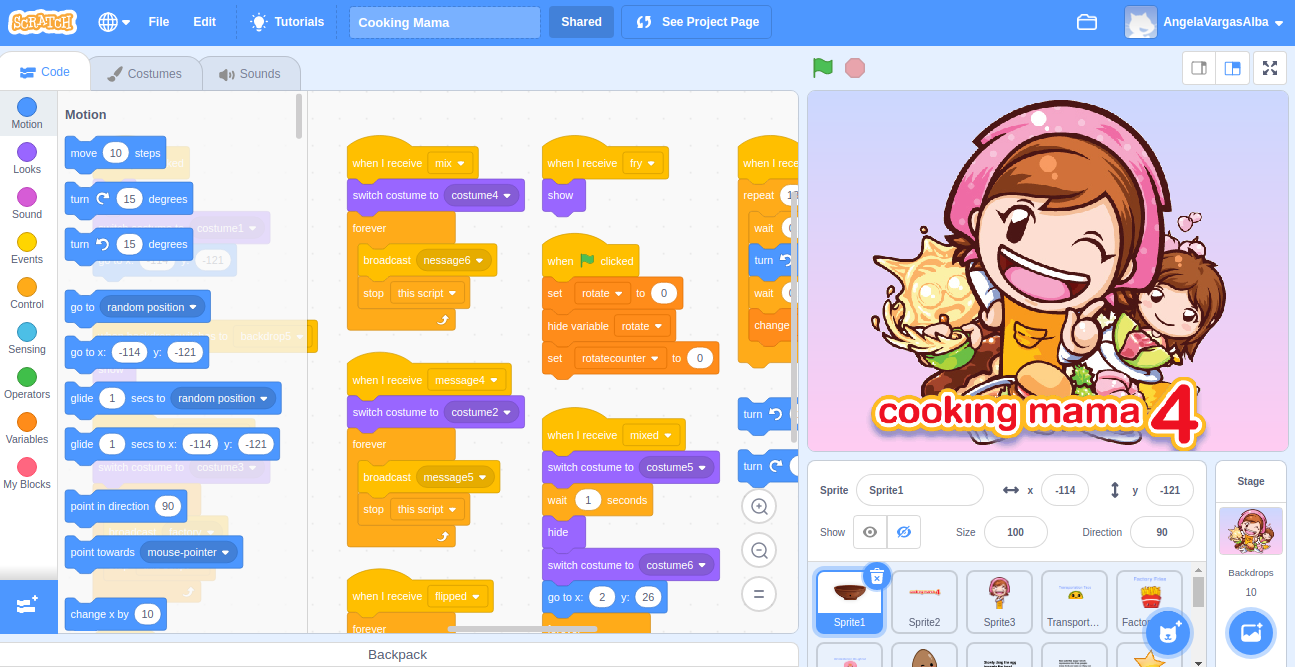
\includegraphics[width=12cm,                         keepaspectratio]{img/cooking_mama.png}
    \caption{\textit{Cooking Mama} project.}
    \label{fig:cooking_mama}
\end{figure}


\subsubsection{Sky Game}
\label{subsubsec:sky_game}

We can appreciate a simpler code than the previous one in Figure~\ref{fig:sky_game}. Even so, there are also numerous names by default in sprites (Sprite5, Sprite6, Sprite7 or Sprite9, among others). In addition, we can find many badly initialized attributes throughout its code. The project is available at \url{https://scratch.mit.edu/projects/366066808/}.

 \begin{figure}
    \centering
    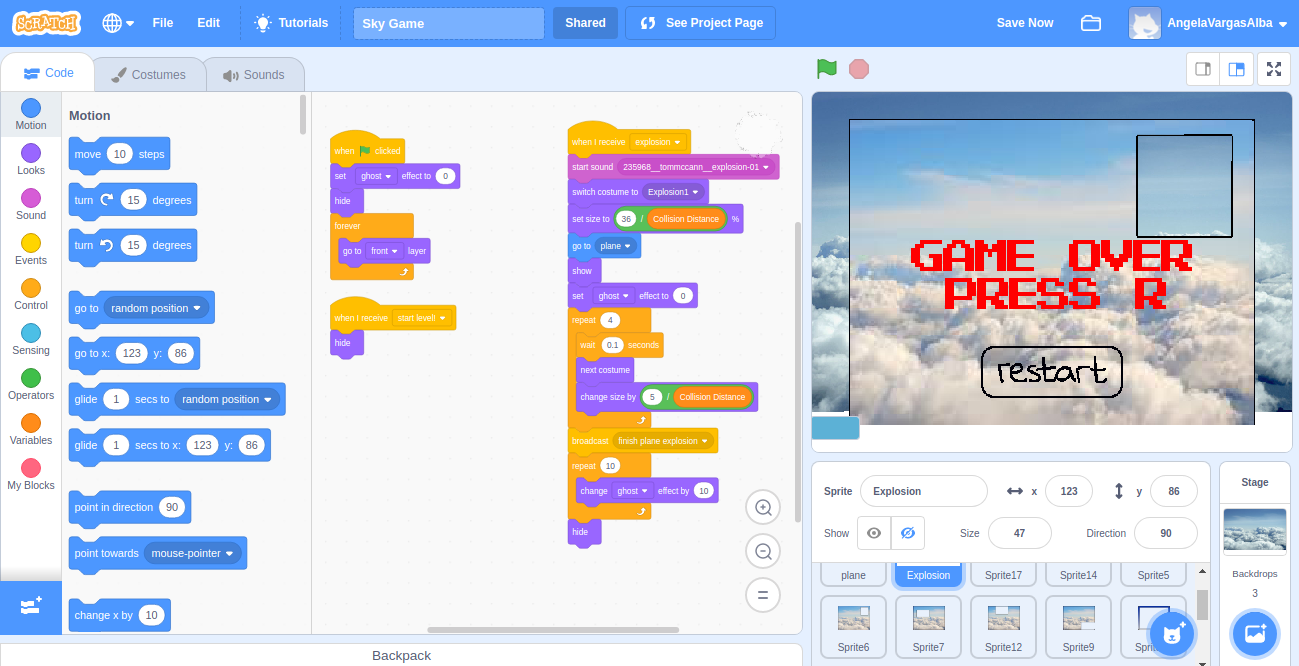
\includegraphics[width=13cm,                         keepaspectratio]{img/sky_game.png}
    \caption{\textit{Sky Game} project.}
    \label{fig:sky_game}
\end{figure}

\subsubsection{Cutting Down}
\label{subsubsec:cutting_down}

In this case, the code of the \textit{Cutting Down} project almost does not have bad smells, according to the assessment of the Dr. Scratch tool. For instance, we can observe personalize names of sprites (tree1, tree2 or tree3, among others) instead of default naming in Figure~\ref{fig:cutting_down}.

However, despite there is only one repeated structure of blocks, it is repeated in many sprites (the code of each \textit{tree} is practically the same), causing the effect of many duplicated code. The project is available at \url{https://scratch.mit.edu/projects/366066161/}.

 \begin{figure}
    \centering
    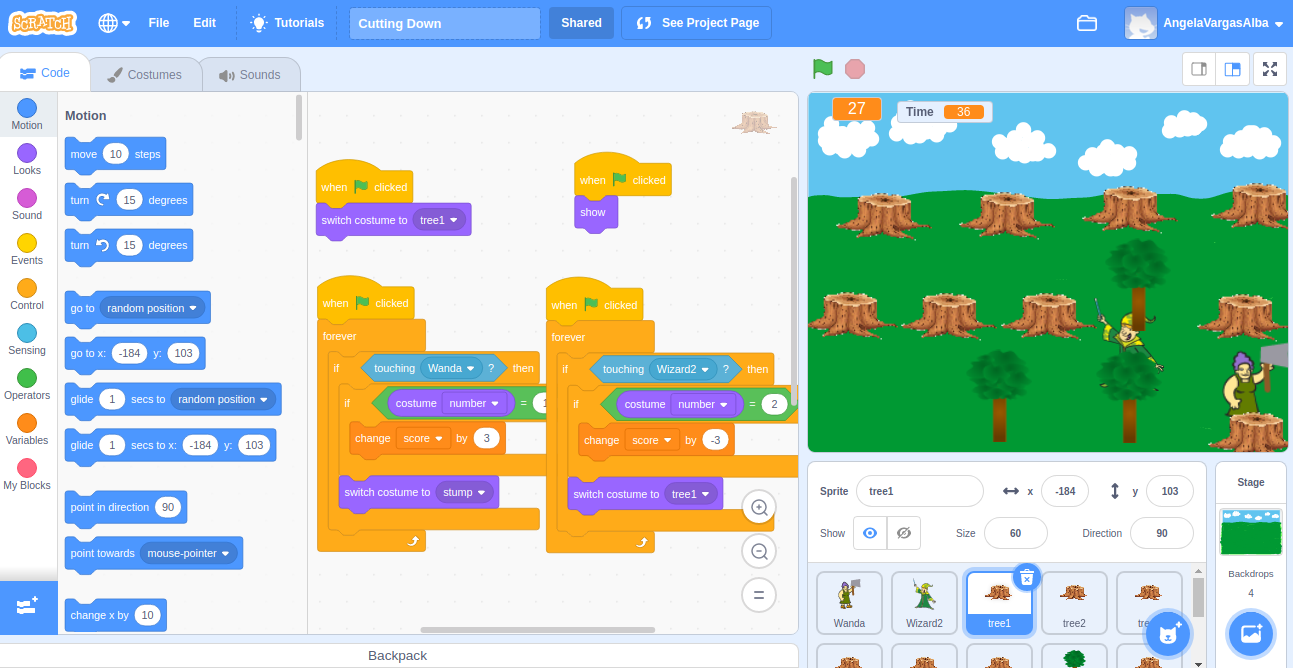
\includegraphics[width=13cm,                         keepaspectratio]{img/cutting_down.png}
    \caption{\textit{Cutting Down} project.}
    \label{fig:cutting_down}
\end{figure}

\subsubsection{Sea Game}
\label{subsubsec:sea_game2}

In Figure~\ref{fig:sea_game} we can observe how in a simple code can appear different bad smells. For instance, the code of the \textit{Sprite2} is mainly composed of repeated blocks, in addition to its default name. Moreover, we can appreciate other names by default, such as \textit{Sprite3, Sprite4} or \textit{Sprite5}, among others. The project is available at \url{https://scratch.mit.edu/projects/366067289/}.

 \begin{figure}
    \centering
    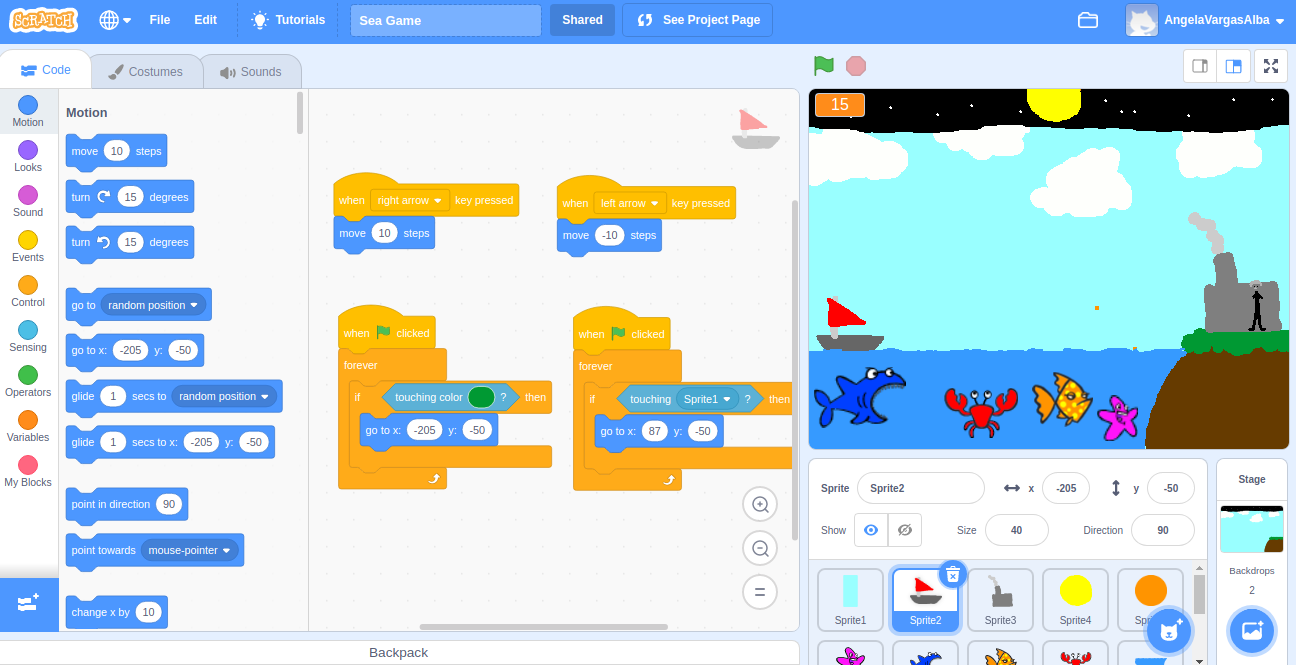
\includegraphics[width=13cm,                         keepaspectratio]{img/sea_game.png}
    \caption{\textit{Sea Game} project.}
    \label{fig:sea_game}
\end{figure}

\subsubsection{Environment Game}
\label{subsubsec:environment_game}

The \textit{Environment Game} project is designed with a simple code. The program is only composed of three sprites, which are defined with personalize names, as we can observe in Figure~\ref{fig:environment_game}. However, the code is repetitive and the richness of blocks is scarce. The project is available at \url{https://scratch.mit.edu/projects/366066063/}.

 \begin{figure}
    \centering
    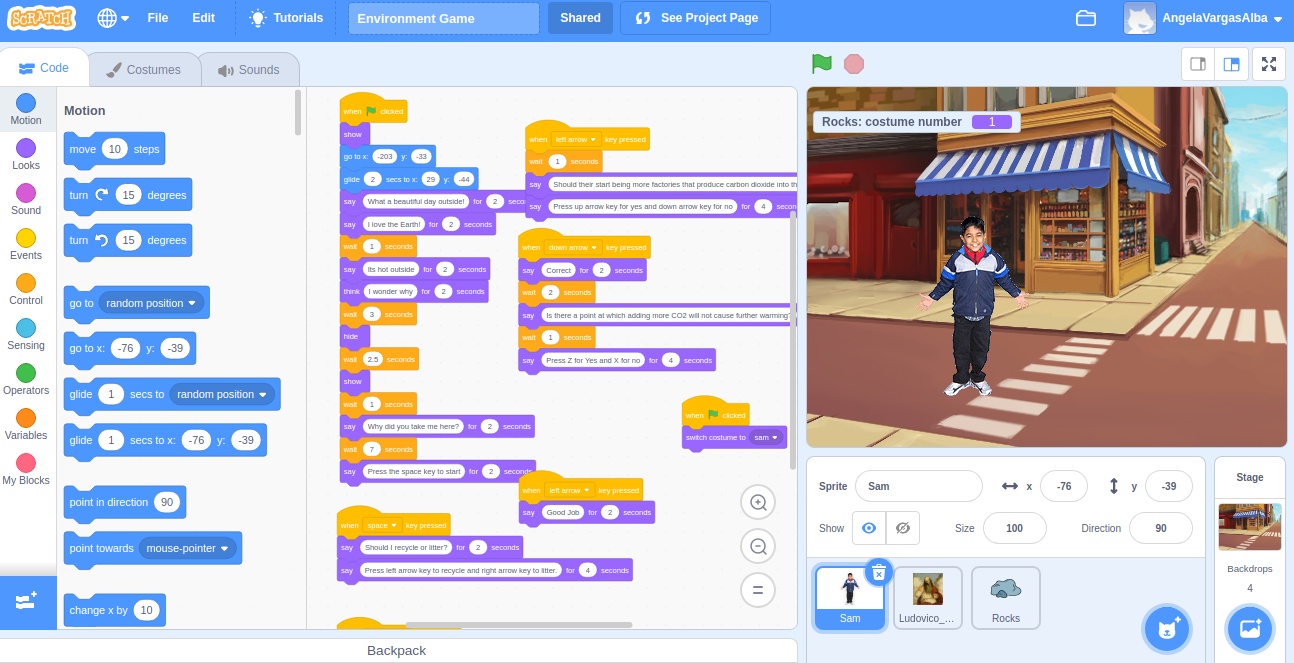
\includegraphics[width=13cm,                         keepaspectratio]{img/environment_game.png}
    \caption{\textit{Environment Game} project.}
    \label{fig:environment_game}
\end{figure}

\subsubsection{Maze Game}
\label{subsubsec:maze_game}

Even though the number of bad smells in this project is almost null in the Dr. Scratch assessment, we can observe the disorder and the quality of its code in Figure~\ref{fig:maze_game}. We can appreciate that the majority of the scripts shares the same block structure and the same functionality. In addition, although the program does not have default naming, it mainly contains repeated sprites (Factory, Factory2, Factory3, \ldots). This project is available at \url{https://scratch.mit.edu/projects/366056709/}.  

 \begin{figure}
    \centering
    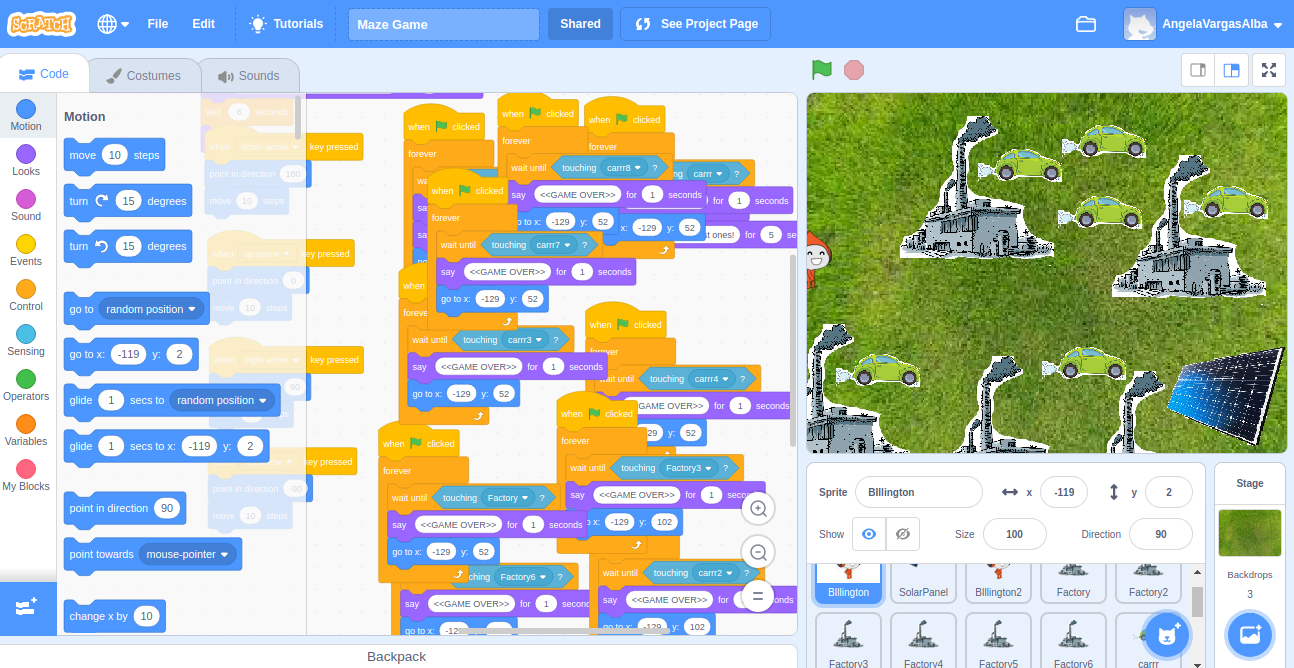
\includegraphics[width=13cm,                         keepaspectratio]{img/maze_game.png}
    \caption{\textit{Maze Game} project.}
    \label{fig:maze_game}
\end{figure}



\section{Phase 1}
\label{app:phase_1}

Regarding the Google Forms, in Figure~\ref{subfig:questions_general_1} we can observe the design of the general questions in the first phase of the experiment described in Chapter~\ref{chap:implementation}. This question is repeated for each project. In addition, in Figure~\ref{subfig:questions_order_1} is shown the last question related to the projects order. 

\begin{figure}
    \begin{subfigure}{.5\textwidth}
    \centering
    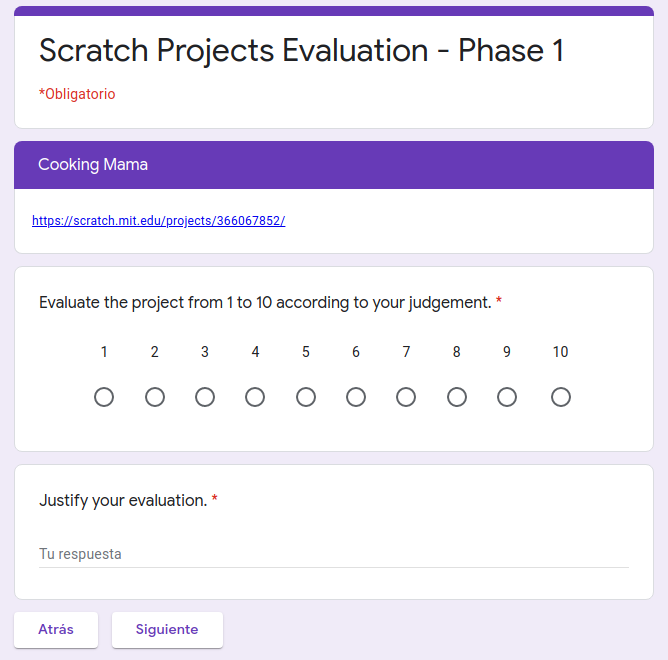
\includegraphics[width=8cm]{img/experiment_question_1.png}
    \caption{General analysis.}
    \label{subfig:questions_general_1}
  \end{subfigure}
  \begin{subfigure}{.5\textwidth}
    \centering
    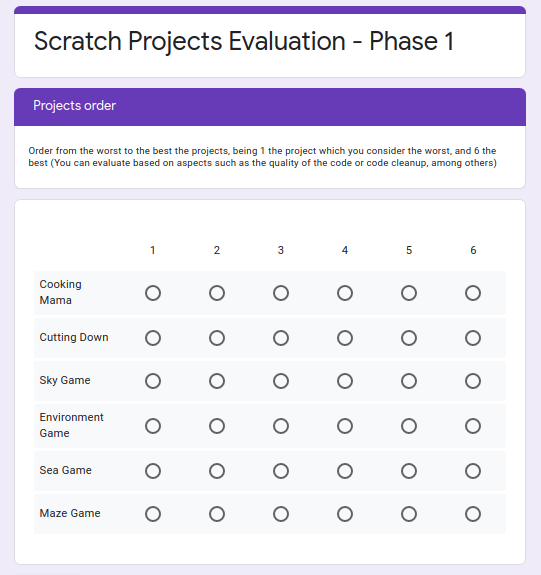
\includegraphics[width=8cm]{img/projects_order_1.png}
    \caption{Projects order.}
    \label{subfig:questions_order_1}
  \end{subfigure}
    \caption{Question design in the first phase of the assessment experiment.}
    \label{fig:question_design_1}
\end{figure}


\section{Phase 2}
\label{app:phase_2}

Lastly, we can observe the design of the questions in the second phase of the experiment in Figure~\ref{fig:question_design_2}. In this case, we guide the evaluation by asking specific aspects of each bad smell. Again, this question is repeated for each project. At the end of the form, the question related to the projects order is included, as we showed in the previous form.

\begin{figure}
    \centering
    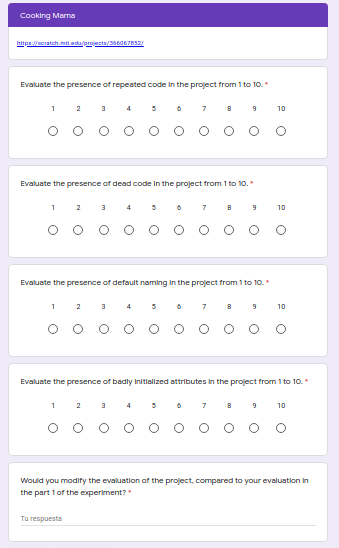
\includegraphics[width=9cm,                         keepaspectratio]{img/experiment_question_2.png}
    \caption{Question design in the second phase of the assessment experiment.}
    \label{fig:question_design_2}
\end{figure}
